\chapter{Modelo matemático}

\section{Modelo cinemático}
\subsection{Matriz de transformación homogénea}



\begin{figure}
    \centering
    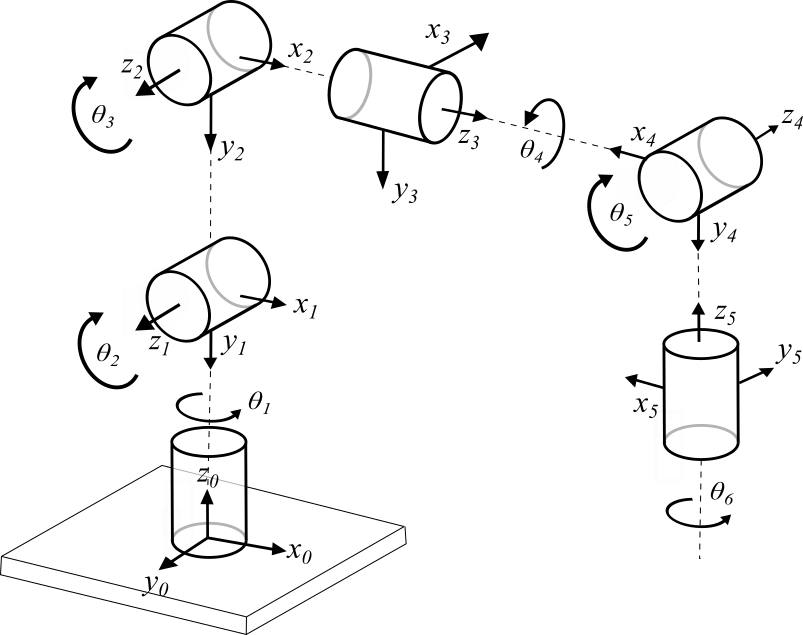
\includegraphics[width=\textwidth]{./img/chapter4/kinematicchainv4.png}
    \caption{Cadena cinemática ¿free body diagram?}
    \label{fig:kinematicchain}
\end{figure}

\[
{}_{0}^{1}T = 
\begin{bmatrix}
    1 & 0 & 0 & 120  \\
    0 & \cos{\theta} & -\sin{\theta} & 0 \\
    0 & \sin{\theta} & \cos{\theta} & 0 \\
    0 & 0 & 0 & 1
\end{bmatrix}
\]
